\section{ОХОРОНА ПРАЦІ І НАВКОЛИШНЬОГО СЕРЕДОВИЩА}
\subsection{Загальні положення}
Охорона праці --- це система правових, соціально-економічних, організаційно-технічних, санітарно-гігієнічних і лікувально-профілактичних заходів та засобів, спрямованих на збереження життя, здоров’я і працездатності людини у процесі трудової діяльності.

Завдання охорони праці полягає в тому, щоб звести до мінімуму ймовірність поразки працюючого під дією небезпечного виробничого фактора або захворювання під дією шкідливого виробничого фактора з одночасним забезпеченням комфортних умов при максимальній продуктивності праці. Закон України <<Про охорону праці>> визначає основні положення по реалізації конституційного права громадян на охорону їх життя і здоров'я в процесі трудової діяльності; регулює взаємини між адміністрацією і працівником в незалежності від форм власності; встановлює єдиний порядок організації охорони праці в Україні [10]. %CITE%

Згідно з Законом України «Про охорону навколишнього середовища» [11] на всіх підприємствах, в установах, організаціях створюються здорові та безпечні умови праці. Чинність Закону поширюється на всі підприємства в Україні, незалежно від форм власності і видів діяльності; на всіх громадян, які працюють, а також залучені до праці на цих підприємствах. % CITE %

Сьогодні комп’ютерна техніка широко застосовується у всіх сферах людської діяльності. Усе більше людей різних професій не можуть обійтися без допомоги комп’ютера. Це не дивно, оскільки розрахунки за допомогою ЕОМ значно допомагають заощадити час і кошти. Тому, необхідно приділяти більше уваги забезпеченню безпечних і нешкідливих умов праці користувачів ЕОМ, підвищити контроль над підтримкою діючих норм, стандартів, правил, інструкцій та інших офіціальних документів по техніці безпеки споруджень, обладнання та машин.

Під час роботи на комп’ютері людина піддається впливові ряду шкідливих і небезпечних факторів, що пов’язано з небезпекою одержання травм і професійних захворювань.

Максимально зменшити кількість шкідливих впливів на людину при високій продуктивності праці, створити комфортні умови для роботи людей --- ось одна з головних задач охорони праці.

Умови праці користувачів ЕОМ повинні відповідати закону про охорону праці.

Питання охорони праці розглядаються для етапу програмування на ЕОМ. Робота проводиться в інформаційно-обчислювальному центрі (ІОЦ), який знаходиться в ТОВ «Тімдев». 

У інформаційно-обчислювальному центрі знаходиться 10 комп’ютерів з 10 робочими місцями. Загальна фактична площа ІОЦ складає 75 $\text{м}^\text{2}$, загальний об’єм приміщення --- 225 $\text{м}^\text{3}$ .

\subsection{Структура управління охороною праці на підприємстві}
У зв’язку з тим, Закон України «Про охорону праці» [10] поширюється на всіх юридичних та фізичних осіб, роботодавець зобов’язаний створити на робочому місці в кожному структурному підрозділі умови праці відповідно до нормативно-правових актів, а також забезпечити додержання вимог законодавства щодо працівників у галузі охорони праці. Із цією метою роботодавець забезпечує функціонування системи управління охороною праці, що окрім всього іншого включає в себе створення відповідних служб на підприємстві та призначення посадових осіб, які забезпечують вирішення конкретних питань.

Система управління охороною праці (СУОП) є комплексом дій з підготовки, прийняття та реалізації рішень з метою виконання організаційних, технічних, санітарно-гігієнічних і лікувально-профілактичних заходів.

Головна мета введення СУОП на розглядаємому підприємстві ТОВ «Тімдев» --- забезпечення безпеки, збереження життя, здоров'я та працездатності працівників під час трудового процесу. Підприємство має наступний склад \ref{tbl:ber_1}.

%Таблиця 5.1 – Структура ТОВ «Тімдев» та його штатній розклад за завданням
\begin{stdtablelong}{4}{|C{2cm}|C{7cm}|C{2cm}|C{5cm}|}
{\label{tbl:ber_1}Структура ТОВ <<Тімдев>> та його штатний розклад за завданням}
{  
Номер за журналом групи
&
Структурні підрозділи
&
Кількість працівників
&
Примітка}
7 & Директор, заст. директора, технічний відділ, відділ реалізації продукції, бухгалтерія, виробнича ділянка. & 20 & Фахівець із охорони праці залучається із іншої організації \\ \hline
\end{stdtablelong}
%

Згідно таблиці \ref{tbl:ber_1} розглянемо структуру управління охороною праці ТОВ «Тімдев» на рисунку \ref{fig:ber_1}.

\begin{stdfigure}
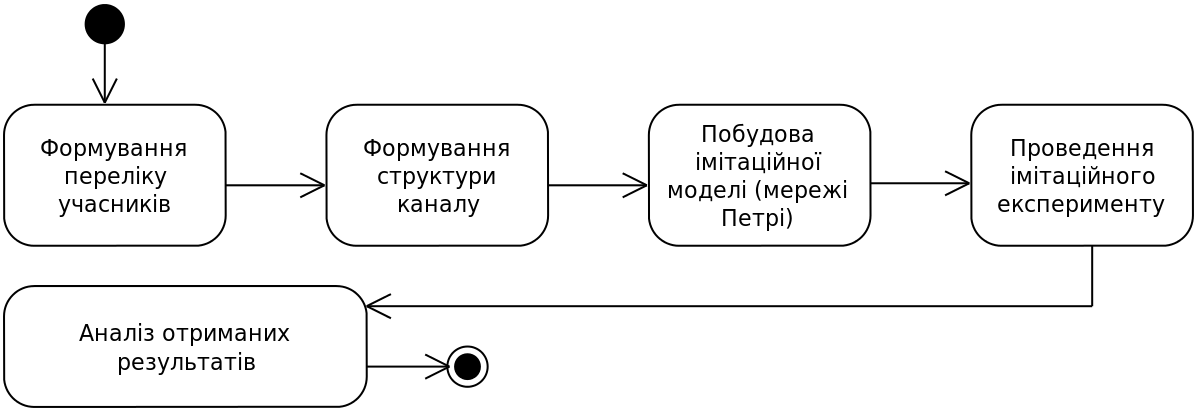
\includegraphics[width=2in]{images/uml_act_solution_schema.png}
\caption{Схема розв’язання задачі в вигляді діаграми активностей}
\label{fig:ber_1}
\end{stdfigure}   

Управління охороною праці здійснюється: на підприємстві у цілому --- директором підприємства безпосередньо та через заступника. У підрозділах та відділах --- керівниками підрозділів. Контроль за дотриманням вимог із питань охорони праці та навколишнього середовища, підготовка звітності, рішень та пропозицій щодо покращення умов праці, виконує фахівець із охорони праці.

\subsection{Характеристики робочого приміщення}

Приміщення, в якому виконувалась науково-дослідна робота --- це інформаційно-обчислювальний центр (ІОЦ). Він знаходиться на сьомому поверсі семиповерхової будівлі, яка споруджена із бетонних конструкцій. Приміщення наведене у таблиці \ref{tbl:ber_2}.

Згідно з НПАОП 0.00-1.28-2010 [12] в лабораторії може перебувати 10 працівників. Мінімальна припустима площа приміщення на 1 людину повинна складати не менш 6,0 $\text{м}^\text{2}$ при роботі з ПЕОМ. За умовами завдання це виконується повністю. В приміщенні відсутні умови, які можуть створювати підвищену або особливо підвищену небезпеку, тому воно відноситься до класу звичайних приміщень (згідно ПУЕ-2011 [13]). Джерелом живлення є трифазна мережа напруги 380/220 В з глухо заземленою нейтралю, з частотою 50 Гц (згідно НПАОП 0.00-1.28-2010 [12]). За пожежо-вибухонебезпекою приміщення лабораторії відноситься до класу В. У таблиці \ref{tbl:ber_3} наведена загальна характеристиака приміщення щодо вибухо-пожежної небезпеки та за важкістю робіт. 

% Таблиця 5.3 – Загальна характеристика приміщень щодо вибухо-пожежної небезпеки та за важкістю робіт
%
%

\begin{stdtablelong}{4}{|C{2cm}|C{5cm}|C{4cm}|C{5cm}|}
{\label{tbl:ber_2} Загальні характеристики умов праці}
{  
Номер за журналом групи
&
Шкідливі та небезпечні фактори на робочому місці
&
Джерела утворювання небезпек
&
Примітка}
7 & Електрична напруга вище 127 В; Шум;  
Випромінювання --- електромагнітні, радіаційні, теплові; 
Статична електрика;
Пожежна небезпека у приміщенні; 
Не якісне освітлення. 
&
Кондиціонер,8-ПЕОМ,Виробнича ділянка, Папір, Світильники (лампи) & Розміри приміщення (м):
Довжина --- 7; 
Ширина --- 5; 
Висота --- 3; 
Кількість працюючих --- 7. \\ \hline
\end{stdtablelong}

\begin{stdtablelong}{3}{|C{5cm}|C{3cm}|C{8cm}|}
{\label{tbl:ber_3} Загальна характеристика приміщень щодо вибухо-пожежної небезпеки та за важкістю робіт}
{  
Характеристика приміщень за вибухопожежною категорією та класом зони
&
Загальна характеристика приміщення
&
Категорія за важкістю робіт згідно ГН 3.3.5-8.6.6.1-2002
}
В-пожежонебезпечна, Клас П-ІІ  & Звичайне, без ознак хімічного забруднення та нормальної вологості за санітарними вимогами &
1а --- до 139 Вт/$\text{м}^\text{2}$ 

1б --- 140-174 Вт/$\text{м}^\text{2}$ 

Клас умов праці: оптимальний. Окремі показники напруженністі трудового процесу – ступінь ризику для власного життя – виключен; ступінь відповідальності за безпеку інших осіб – виключено.

Ступінь відповідальності за результат своєї діяльності. Значущість помилки: допустимий. Напруженність праці середнього ступеня, а саме --- несе відповідальність за функціональну якість допоміжних завдань. Вимагає додаткових зусиль з боку керівництва (керівника дипломної роботи); спостереження за екраном відеотерміналу (годин на зміну) 2-3.
 \\ \hline
\end{stdtablelong}

\subsection{Мікроклімат виробничого приміщення}
Мікроклімат --- метеорологічні умови внутрішнього середовища приміщень, які визначаються діючими на людину сполученнями температури, відносної вологості, швидкості руху повітря й теплового випромінювання.

Під час роботи з ПЕОМ необхідно дотримувати оптимальні метеорологічні умови. Оптимальні метеорологічні умови - сполучення параметрів, які при тривалому й систематичному впливі на людину забезпечують збереження нормального функціонального й теплового стану організму без напруження реакцій терморегуляції. Параметри  мікроклімату  в  приміщенні  повинні  відповідати ГОСТ 12.1.005-88 [14]. Із урахуванням категорії роботи за енерговитратами повинні дотримуватися параметри мікроклімату, наведені в \ref{tbl:ber_4}.

%Таблиця 5.4 - Оптимальні параметри мікроклімату 
%
%

Для підтримки в приміщенні оптимального температурного режиму відповідно до вимоги СНиП 2.04.05-92 [15] передбачена система опалення (загальне парове) в холодному періоді, та вентиляція (загальна приточно-витяжна штучна), кондиціювання та регулювання вологості повітря в теплому.

\subsection{Виробниче освітлення}

Особливістю роботи за дисплеєм ЕОМ є постійна й значна напруга функцій зорового аналізатора, обумовленого необхідністю розходження самосвітних об'єктів (символів, знаків і т.п.) при наявності відблисків на екрані, рядковій структурі екрана, мерехтіння зображення, недостатньою чіткістю об'єктів розходження.

Для забезпечення нормального освітлення застосовуються природне бокове одностороннє й штучне освітлення, які нормуються ДБН В.2.5-28-2006 [16] та НПАОП 0.00-1.28-2010 [12].

По характеру зорової роботи, робота відноситься до високої точності, розряд зорової роботи III, підрозряд. Раціональне освітлення приміщення сприяє кращому виконанню виробничого завдання і забезпеченню комфорту при роботі. Для забезпечення нормального освітлення застосовуються природне, однобічне, бічне і штучне освітлення, а також сполучене, які нормуються санітарними нормами й правилами ДБН В.2.5-28-2006 [16]. Дані по нормах освітлення наведені в \ref{tbl:ber_5}.

%Таблиця 5.5 - Норми природного й штучного освітлення
%
%

Відділ забезпечений комбінованим освітленням. В темний час доби передбачається загальне і/або місцеве рівномірне штучне, а в світлий --- бокове одностороннє природне освітлення два віконних прорізи.

Для розміру об'єкту розрізнення 0,3---0,5 мм (III розряд зорової роботи) світлового фону і середнього контрасту об'єкту розрізнення з фоном (підрозряд «г») нормоване значення коефіцієнта КПО ен = 1,5\%. Мінімальна освітленість $\text{Е}_\text{min}$=300 лк, підтримується за рахунок кількості та потужності електроламп.

Штучне освітлення виконано за системою загального освітлення, коли освітлюється рівномірно все приміщення, і за системою комбінованого освітлення, коли, окрім загального освітлення на робочих місцях встановлюється світильники місцевого освітлення, що створюють підвищену освітленість робочих місць.

\subsection{Промисловий шум та вібрації}
Одним з найбільш поширеніших чинників зовнішнього середовища, який несприятливо впливає на людину, є шум.

Шум погіршує умови праці здійснюючи шкідливу дію на організм людини. Працюючі в умовах тривалої шумової дії випробовують дратівливість, головні болі, запаморочення, зниження пам'яті, підвищену стомлюваність, пониження апетиту, болі у вухах і т.д. Такі порушення в роботі ряду органів і систем організму людини можуть викликати негативні зміни в емоційному стані людини аж до стресових ситуацій. Під впливом шуму знижується концентрація уваги, порушуються фізіологічні функції, з'являється стомленість у зв'язку з підвищеними енергетичними витратами і нервово-психічною напругою, погіршується мовна комутація. Все це знижує працездатність людини і її продуктивність, якість і безпеку праці. Тривала дія інтенсивного шуму [вище 80 дБ] на слух людини приводить до його часткової, або повної втрати. 

У приміщенні технічного відділу причинної шуму і вібрації являються апарати, прилади і устаткування: друкуючі пристрої, комп'ютери, вентилятори, кондиціонер та ін. При їхній роботі рівень вібрації не вище 33 дБ, рівень шуму не повинен перевищувати 50 дБА, що є нормою для даного виду діяльності відповідно до ГОСТ 12.1.003-83* [17] та НПАОП 0.00-1.28-2010 [12]. Заходи по забезпеченню встановлених норм: використання спеціальних шумопоглинаючих перегородок, застосування меблів, які сприяють зменшенню шуму і вібрації, установка апаратів і приладів на спеціальні амортизуючи підкладки.

\subsection{Електробезпека}
Електробезпека --- це система організаційних та технічних заходів і засобів, що забезпечують захист людей від небезпечних і шкідливих дій електричного струму і електричного поля. Основну небезпеку, для працюючих в відділі, представляє напруга електромережі в електроприладах, та ЕОМ.

Персональна ЕОМ є однофазним споживачем електроенергії від трифазної чотири ядерної мережі змінного струму з глухо заземленою нейтраллю, напругою 380/220 В, частотою 50 Гц.

Основними заходами захисту від ураження електричним струмом є:
\begin{longEnumerate}
\item конструктивні заходи (ПК відноситься до електроустановок до 1000 В закритого виконання, всі токоведучі частини знаходяться в кожухах [17]. Ступінь захисту персоналу від зіткнення зі струмоведучими частинами усередині захисного корпуса і від улучення води усередину корпуса ІР-44, де перша <<4>> --- захист тіл, розміром більш 1,0 мм, друга <<4>> --- захист від бризгів води);
\item в якості схемно-конструктивного заходу безпеки застосовується занулення – навмисне з’єднання металевих частин комп’ютера, що у випадку аварії можуть виявитися під напругою, з нейтраллю;
\item експлуатаційні міри (необхідно дотримуватися правила техніки безпеки при роботі з високою напругою, а також наступної міри обережності не підключати і не відключати рознімання кабелів при включеній напрузі мережі, технічне обслуговування і ремонт робити тільки при вимкнутому живленні).
\end{longEnumerate}

\subsection{Пожежна безпека}

За категорією вибухопожежонебезпечності згідно НАПБ Б.03.002-2007 [18] приміщення ІОЦ відноситься до категорії Д-пожежонебезпечне, бо на ІОЦ є негорючі речовини і матеріали у холодному стані (робочі столи, папір, ізоляція та ін.). З урахуванням категорії вибухопожежонебезпечності, етажності будівлі та матеріалу конструкцій (бетону) встановлений II ступінь вогнестійкості будівлі згідно ДБН В 1.1-7-02 [19].

Пожежна безпека відповідно до ГОСТ 12.1.004-91 [20]  забезпечується наступними нормами:
\begin{itemize}
\item системою запобігання пожежі;
\item системою пожежного захисту;
\item організаційно-технічними заходами щодо пожежної безпеки.
\end{itemize}

У помешканні відділу сухо, відносна вологість 48-55\%, температура повітря перевищує 27°С. По категорії вибухо- і пожежонебезпеки дане помешкання відноситься до категорії В-пожежонебезпечності через присутність твердих згораючих матеріалів, таких як: робочі столи, ізоляція, папір та інше. Виходячи з категорії пожежонебезпеки і поверховості будинку ступінь вогнестійкості будинку друга [21].

Система запобігання пожежі:
\begin{enumerate}
\item контроль і профілактика ізоляції;
\item наявність плавких вставок і запобіжників в електронному устаткуванні;
\item для захисту від статичної напруги використовується заземлення;
\item захист від блискавки будинку і устаткування.
\end{enumerate}

Система пожежного захисту:
\begin{enumerate}
\item аварійне відключення і переключення апаратури; 
\item наявність первинних засобів пожежогасіння, вогнегасників ВВК-5, тому що вуглекислота має погану електропровідність, або порошкових вогнегасників;
\item система оповіщення, світлова і звукова сигналізація; захист легкозаймистих частин устаткування, конструкцій захисними матеріалами;
\item у помешканнях, де немає робочого персоналу встановлена автоматична система пожежного захисту.
\end{enumerate}

У відділі встановлено 8 вогнегасників типу ВВК-1,4  із розрахунків 1
вогнегасника на 20 $\text{м}^\text{2}$.

Організаційні заходами протипожежної профілактики: є вступний інструктаж під час вступу на роботу, навчання персоналу правилам пожежної безпеки; видання необхідних інструкцій і плакатів, засобів наочної агітації, плану евакуації персоналу у випадку пожежі.

Характеристики пожежної безпеки приміщення наведені у таблиці \ref{tbl:ber_5}.

%Таблиця 5.5 – Характеристики пожежної безпеки приміщення
%

\subsection{Ергономічні вимоги до робочого місця}
Робоче місце оператора ЕОМ обладнується робочим столом, кріслом і підставкою для ніг. Висота робочого стола регулюється в межах 0,68—0,80 м, а при відсутності такої можливості має складати 0,72 м. Мінімальна ширина стола 0,6 м, поверхня стола не блискуча. Робоче крісло оператора забезпечується підіймально-поворотним пристроєм з регулюванням висоти сидіння та спинки. Розміри підставки для ніг довжина 0,4 м, ширина не менше 0,30 м.  На одного працюючого з урахуванням роботи з ПЕОМ має відводитись не менше 6,0 м2 та не менше 20 м3 об’єму приміщення згідно (НПАОП 0.00-1.28-2010 [12]).

\subsection{Охорона навколишнього середовища}
Охорона навколишнього середовища --- це сукупність законодавчих актів, соціально-економічних, профілактичних і організаційно-технічних заходів, що запобігають забрудненню біосфери: земельних та водних ресурсів, а також атмосфери --- шкідливими викидами.

Охорона навколишнього природного середовища, раціональне використання природних ресурсів, забезпечення екологічної безпеки життєдіяльності людини --- невід'ємна умова сталого економічного та соціального розвитку України. З цією метою Україна здійснює на своїй території екологічну політику, спрямовану на збереження безпечного для існування живої і неживої природи навколишнього середовища, захисту життя і здоров'я населення від негативного впливу, зумовленого забрудненням навколишнього природного середовища, досягнення гармонійної взаємодії суспільства і природи, охорону, раціональне використання і відтворення природних ресурсів.

Закон України «Про охорону навколишнього природного середовища» [11] визначає правові, економічні, соціальні основи охорони навколишнього середовища та регулювання відносин в області охорони природи, використанні й відтворенні природних ресурсів, забезпеченні й ліквідації наслідків негативного впливу на навколишнє середовище господарської й іншої діяльності людини, збереження природних ресурсів, генетичного фонду нації, ландшафтів та інших природних об’єктів.

При масовому використанні моніторів і комп’ютерів не можна не врахувати їх вплив на навколишнє середовище на всіх стадіях: при виготовленні, експлуатації та після закінчення їх терміну служби. Сьогодні діють екологічні стандарти, які визначають вимоги до виробництва і матеріалів, що використовуються в конструкції приладів. Вони не повинні містити фреонів, хлоридів, бромідів і полівінілхлориду (ТСО’95 [22], BS7750 [23]). ТСО’95 включають вимоги зниженого енергоспоживання і обмежують допустимі рівні потужності, споживані в неактивному стані.

У стандартах ТСО’95 закладено обмеження з кадмію в світлочутливому шарі екрану дисплея і ртуті в батареях. Апарати, тара і документація повинні допускати нетоксичну переробку після використання.

Міжнародні стандарти з ТСО’95 включають вимоги зниженого енергоспоживання і обмеження допустимих рівнів потужності, споживаних в неактивному режимі.

Всі комп’ютери встановлені в даному приміщені були виготовлені не раніше 2007-го року. Монітори відповідають міжнародним стандартам [22]. Комп’ютери відповідають стандарту (ISO 9001 [24]). Робота на ПК не надає шкідливої дії на навколишнє середовище. Після закінчення терміну служби він повністю підлягає вторинній переробці, а також апарати, тара, документація повинні допускати нетоксичну переробку після використання.

Висновок: В ТОВ «Тімдев» повністю забезпечене створення здорових, безпечних умов праці т покращення виробничого побуту. Для покращення умов праці було установлено новітню систему вентиляції та опалення; дотримано вимоги до комплектації робочого місця; фактичні рівні шуму не перевищують нормативних значень. Пожежна безпека забезпечується системами запобігання пожежі, пожежного захисту, організаційно-технічними заходами. У відділі встановлено пожежну сигналізацію, а також первинні засоби захисту від пожежі, у виді 3-ми вогнегасників типу ВВК-1,4.


